\documentclass[paper=a4, fontsize=11pt]{article}
\usepackage[T1]{fontenc}
\usepackage{fourier}

\usepackage[english]{babel}															% English language/hyphenation
\usepackage[protrusion=true,expansion=true]{microtype}	
\usepackage{amsmath,amsfonts,amsthm} % Math packages
\usepackage[pdftex]{graphicx}	
\usepackage{url}
\usepackage{geometry}
\usepackage{listings,multicol} % listings to include code samples
\usepackage{xcolor} % to change color in code listings

\usepackage{caption}
\usepackage{cleveref}

%%% Equation and float numbering
\numberwithin{equation}{section}		% Equationnumbering: section.eq#
\numberwithin{figure}{section}			% Figurenumbering: section.fig#
\numberwithin{table}{section}				% Tablenumbering: section.tab#


%hyphenation
\hyphenation{back-logs}
\newcommand*\idstyle{%
         \expandafter\id@style\the\lst@token\relax
 }
% set parameters for lstlisting and lstinline
\lstset{
  breaklines=true, % Enables wrapping in lstlisting environment.
  backgroundcolor=\color[HTML]{F8F8F8},
  frame=tlrb,
  language=Ruby,
  keepspaces=true, 
  framextopmargin=5pt,
  framexleftmargin=5pt,
  framexrightmargin=5pt,
  framexbottommargin=5pt,
  commentstyle=\itshape\color[HTML]{999988},
  rulecolor=\color[HTML]{DDDDDD},
  stringstyle=\color[HTML]{dd1144},
  keywordstyle=\color[HTML]{990000},
  identifierstyle=\color[HTML]{333333},
  morecomment=[l]{//},
  morecomment=[s]{/*}{*/},
  keywords={if, else, elseif, do, end, while, const, def, begin, func, and, or, {||}, {&&}},
  keywordstyle=\color[HTML]{333333}\bfseries, 
  % numbers=left, %we need line numbers to make line wrapping obvious
  numberstyle=\color[HTML]{888888}, %we want line numbers to blend in
  tabsize=4,
  literate={`}{${}^\backprime$}1
           {_}{$\_$}1
           {"}{\textquotedbl}1
           {'}{\textquotesingle}1
}
\renewcommand{\lstlistingname}{Code}

\lstdefinestyle{muchcode}{
  numbers=left, %we need line numbers to make line wrapping obvious
  numberstyle=\color[HTML]{888888} %we want line numbers to blend in
}
\lstdefinestyle{densecode}{
  aboveskip=1cm,
  belowskip=1cm,
  xleftmargin=-1.85cm, % Alters margin for listings to fit more code on a line.
  xrightmargin=-1.85cm, % Alters margin for listings to fit more code on a line.
  basicstyle=\small\ttfamily,
  numbers=left, %we need line numbers to make line wrapping obvious
  numberstyle=\color[HTML]{888888} %we want line numbers to blend in
}
\lstdefinestyle{densecodenomargins}{
  aboveskip=1cm,
  belowskip=1cm,
  xleftmargin=0.8cm, % Alters margin for listings to fit more code on a line.
  xrightmargin=0.3cm, % Alters margin for listings to fit more code on a line.
  basicstyle=\footnotesize\ttfamily,
  numbers=left, %we need line numbers to make line wrapping obvious
  numberstyle=\color[HTML]{888888} %we want line numbers to blend in
}
\lstdefinestyle{densecodecolumn}{
  aboveskip=0cm,
  belowskip=0cm,
  xleftmargin=0.8cm, % Alters margin for listings to fit more code on a line.
  xrightmargin=0.3cm, % Alters margin for listings to fit more code on a line.
  basicstyle=\footnotesize\ttfamily,
  numbers=left, %we need line numbers to make line wrapping obvious
  numberstyle=\color[HTML]{888888} %we want line numbers to blend in
}

\lstdefinelanguage{Assembly}{
  keywords={getstatic, loadvirtual, loadstatic, invokestatic, invokespecial, invokevirtual},
  keywordstyle=\color[HTML]{333333}\bfseries, 
  sensitive=false,
  comment=[l]{//},
  tabsize=2,
  morecomment=[s]{/*}{*/},
  commentstyle=\color{purple}\ttfamily,
  stringstyle=\color{red}\ttfamily,
  morestring=[b]',
  morestring=[b]"
}

%%% Maketitle metadata
\newcommand{\horrule}[1]{\rule{\linewidth}{#1}} 	% Horizontal rule

\title{
		%\vspace{-1in} 	
		\usefont{OT1}{bch}{b}{n}
		\normalfont \normalsize \textsc{University of Twente} \\ [25pt]
		\horrule{0.5pt} \\[0.4cm]
		\huge Alia Programming Language \\
		\horrule{2pt} \\[0.5cm]
}
\author{
		\normalfont 								\normalsize
        Fedor Beets\\[-3pt]						\small
        s1227874\\[-3pt]        				\small
        Campuslaan 27\\[8pt]					\normalsize
        Joost van Doorn\\[-3pt]					\small
        s1095005\\[-3pt]						\small
        Dalsteindreef 2404, Diemen\\[8pt]			\normalsize
        \today
}
\date{}


%%% Begin document
\begin{document}
\maketitle
\newpage
\section*{Introduction}
The Alia programming language was built for the final project of the compiler construction course at the University of Twente. In this final project a programming language is specified and implemented in antlr (ANother Tool for Language Recognition). A compiler is built to translate code into a type of machine instructions. The type of machine instructions can vary from language to language. Over the first half of compiler construction course several parts of the design process of building a compiler are individually learned and tested. In the final project this is brought to culmination by going through the entire process from the specification, to in the end a usable programming language. 

This document serves as a specification of the Alia Programming Language (Alia for short) as well as an explanation of the inner workings of the Alia compiler. In it we will give a short description of the Alia Programming Language in the context of programming languages, explain some of the problems faced during the construction of the Alia compiler,  and our solutions. Give a specification of the Alia language with the help of the syntax, context-constraints and semantics. Also in this document are the transformations that show how the symbols of the language are turned into JVM instructions, a description of all the auxiliary Java code made for the compiler. A set of tests is described to give confidence in the correctness of the compiler. Lastly conclusions are drawn from the project.

The Alia source code repository is located at:
\url{https://github.com/JoostvDoorn/VertalerbouwEindproject}

\section{Alia Programming Language}
%De programmeertaal
%Maximaal een A4
The Alia programming language is an expression language with type inference. Alia code is compiled to Java bytecode using Jasmin and can be run using the Java Virtual Machine (JVM). As an expression language every statement has a return type. Functional statements such as print, read and conditional statements all return values. For example the print function may return a value which can be used in an assignment statement.

\begin{lstlisting}
x = print(34) + 1 // x is assigned 35
\end{lstlisting}

Alia contains compound statement which are a series of statements with the last statement as return value, compound statements are used in conditional statements and can be explicitly used for scoping.

\begin{lstlisting}
x = begin
    y = 3 // Only declared in this scope
    y + 1 // Return value for the compound statement
end
if y = true; y && x < 10 do // y here has a different scope
    print(y) // Print the value of y
    print('t')
end
\end{lstlisting}

Types in Alia are inferred and do not need explicit declarations. Types can be declared explicitly within an assignment statement, but are not required. In the current form of the programming language, type inference can always deduce the type of a declaration. However in an extended version of Alia with functions and procedures, explicit type declarations will be required in cases where type inference will not be able to deduce the type of the variable or function return type. Type inference makes programming easier, it reduces the work of the programmer by making explicit type declarations optional, and reduces the amount of code required for variable declarations. Type checking is maintained and the programmer still has the option to add type declarations if it helps clarify the code.

\begin{lstlisting}
x = 54 : int // x is assigned 54, and is explicitly declared as an int
\end{lstlisting}


%Typer inference
%Expression language

\section{Problems and solutions}
During the construction of the Alia compiler we ran into some problems, as is to be expected during any first time construction of a compiler. In this section we will explain some of the bigger problems that we faced as well as the solutions that we applied.

\subsection{Scope definition}
Because we do not have explicit declarations we cannot redefine a variable inside a new scope. There would be no way to distinguish between redefining a variable in a new scope and reassigning the value that was given to a variable to be used later. With a new variable that overwrites an old one for a temporary scope you would need to assign a new space in memory. We have decided that we want this in our programming language, this is because if you can redeclare a variable inside a new scope then you are only making it more confusing for yourself as a coder. On the other hand not being able to assign a new value to a variable in a new scope destroys a large part of the functionality of language. For these reasons we have chosen to leave it as is.

\subsection{String template expressions}
StringTemplate does not allow you to evaluate an expression inside of a string template. This was purposefully implemented to stop you from putting a large part of the logic in the string template itself. The problem that we have with this is that there are issues that are specific to the creation of java bytecode that must now be evaluated in the antlr part of the program, and must be passed in the creation of any possible target platform. The first time this became a problem was what instructions to use for outputting any given number. A naive solution to this would be to always use the instruction for loading a large number like an integer. But java has special instructions for loading the numbers -1 through 5 and loading smaller numbers that fit on a byte or a short, so we wanted to use these. To solve this issue we created a function that calculated what type a number can fit into in the CodeGeneratorAux class which passes a number of booleans wrapped in a NumberType to the string template. We then use conditional templates to emit different instructions depending on the number to be put on the stack.

%todo: Andere nadelen aan String templates. Geeft geen duidelijke plaatst binnen ANTLR voor java code. Het is lastiger om code repetitie te voorkomen (Do not repeat yourself).

\subsection{Constants}
We chose to put the optimization of replacing all constants by their actual reference in the checker stage. The choice was made because in the checker there is already a list of declared variables, and Java functions to do this. This made it very easy to implement this feature in the checker, and much more ugly to implement in the code generation. In an ideal world there would be a separate stage in-between the checker and the code generation that optimizes the abstract syntax tree, but this one feature was easily done in the checker. We have also chosen to not support constants that can vary, being defined by another identifier. In the Alia programming language a constant can only be defined by a single primitive type.


%uitleg over de wijze waarop je de problemen die je bent tegengekomen bij het maken van de opdracht hebt opgelost (maximaal twee A4-tjes)

\section{Syntax, context-constraints and semantics}
The syntax of Alia is defined as follows:

\begin{verbatim}
program = (func_def | (statement end_statement) | \n)*;

statements = (statement (end_statement statements)? | \n statements)?;
statements_cond = (statement (end_statement statements)? | \n statements_cond )?;

statement = (expr_assignment | const_assignment) (; type)?
			| while_stmnt 
			;

end_statement = \n | ";" | EOF;

expr_assignment = (identifier "=") expr_assignment
				| expr 
				;

const_assignment = CONST identifier "=" primitive;

expr = expr1 ((or | "||") expr1)*;
expr1 = expr2 ((and | "&&") expr2)*;
expr2 = expr3 ((">" | ">=" | "<" | "<=" | "==" | "!=" )^ expr3)*;
expr3 = expr4 (("+" | "-")^ expr4)*;
expr4 = expr5 (("*" | "/" | "%")^ expr5)*;
expr5 = "!" operand | operand | expr_minus | expr_plus;
expr_minus = "-" operand;
expr_plus = "+" operand;
operand = read |
	   	  print |
	   	  if_stmnt |
	   	  "(" expr ")" |
	   	  compound_stmnt |
	   	  primitive |
	   	  func_identifier
		;
		  
compound_stmnt = begin statements end;

primitive = number | character | boolean;

func_identifier = identifier ( "(" exprlist? ")" )?;

while_stmnt = WHILE statements_cond DO statements END;

if_stmnt = IF statements_cond DO statements else_stmnt? END;

else_stmnt = ELSEIF statements_cond DO statements else_stmnt?
			| (ELSE statements)
			;

print = PRINT "(" exprlist ") ;
read = READ "(" varlist ") ;

varlist = identifier ("," identifier)*;
exprlist = expr ("," expr)*;

func_def = DEF identifier "(" varlist ")";
\end{verbatim}


\subsection*{Semantics and context constraints:}
The semantics and context constraints are defined using the abstract syntax of the Alia language.
\paragraph{Program}
\begin{verbatim}
program = ((statement end_statement) | \n)*;
\end{verbatim}
A program is run by executing a sequence of statements.
\paragraph{Statement}
\begin{verbatim}
statements = (statement (end_statement statements)? | \n statements)?;
statements_conditional = (statement (end_statement statements)? | \n statements_cond )?;
end_statement = \n | ";" | EOF;
statement = while_stmnt 
			| (expr_assignment | const_assignment) 
			;
while_stmnt = WHILE statements_cond DO statements END;
if_stmnt = IF statements_cond DO statements else_stmnt? END;
else_stmnt = ELSEIF statements_cond DO statements else_stmnt?
			| (ELSE statements);
compound_stmnt = begin statements end;
\end{verbatim}
\begin{itemize}
\item A statements is a set of statements separated by an end statement.
\item A conditional statements is a statements that is meant for conditional expressions.
\item A statement can be ended by any of the above separators ($\textbackslash n$, $;$, $EOF$).
\item The while statement 'while S1 do S2 end' is executed as follows. The statement S1 is evaluated, if its value is true then S2 is evaluated and the while statement is run again. If the value of S1 is false then the execution is completed. S1 must be of type boolean. This statement is of type void. Declarations made in S1 are valid in S1 and S2. The scope of declarations made in S2 is only S2.

\item If statements of the form 'if S1 do S2 (elseif S3 do S4)* (else S5)?' are executed as follows. S1 is executed. If S1 is true, then S2 is evaluated. If S1 is false and there is an S3, then S3 is evaluted and if true S4 is executed. If the evaluated S3 is false there is another elseif statement then it is evaluated, same as an if statement is. If S1, S3 and all other elseifs have evaluated to false, then S5 is executed. If there is no S5, execution has completed. The type os S1 and S3 must be boolean. If there is no else part, the type of the statement is void. If there is an else part, then if all S2, S4, S5 are the same type, then that is the type of the conditional statement. If S2, S4, S5 are not of the same type then the type of the statement is void. Special scope rules apply, a declaration in S1 or any S3 is valid in S2, S4, S5 as long as the declaration precedes the use. 
\item A compound statement is a closed set of statements. Any assignments made in the statements can not be used outside of the compound statement. The result and type of the compound statement are the same as the last statement in the compound statement.

\end{itemize}
\paragraph{Assignment}
\begin{verbatim}
expr_assignment = identifier "=" expr_assignment
				| expr (: type)?
				;

const_assignment = CONST identifier "=" primitive (: type)?
\end{verbatim}

\begin{itemize}
\item An expression assignment binds one or more identifiers to a value yielded by an expression E. If a type is included then the type and the type of the expression must match. The identifiers can thereafter be used in applied occurrences. The expression assignment yields the value of the expression.
\item The expression 'const I = P (:T)?' is executed as follows. I is bound to the value P. If T was included, T and E must be of the same type. The expression is of type P. I can be used in applied occurrences. I can not be assigned a different value at a later time.
\end{itemize}

\paragraph{Expressions}
\begin{verbatim}
expr = expr1 ((or | "||") expr1)*;
expr1 = expr2 ((and | "&&") expr2)*;
expr2 = expr3 ((">" | ">=" | "<" | "<=" | "==" | "!=" )^ expr3)*;
expr3 = expr4 (("+" | "-")^ expr4)*;
expr4 = expr5 (("*" | "/" | "%")^ expr5)*;
expr5 = "!" operand | operand | expr_minus | expr_plus;
expr_minus = "-" operand;
expr_plus = "+" operand;
\end{verbatim}
\begin{itemize}
\item The expressions 'or', '||', 'and', '\&\&' preceded by E1 and followed by E2 are evaluated by performing a logical or (True iff E1 or E2) in case of 'or' and '||'. In the case of 'and' and '\&\&' it is evaluated by performing a logical and on the two expressions (True iff E1 and E2). E1 and E2 must be of type boolean. The type of the expression is Boolean. These are the logical operators. 
\item The expression 'E1 == E2' is true iff E1 equals E2. 'E1 != E2' is true iff E1 is not equal to E2. 'E1 <= E2' true iff E1 is smaller than or equal to E2. 'E1 >= E2' is true iff E1 greater than or equal to E2. 'E1 > E2' is true iff E1 is greater than E2. 'E1 < E2' is true iff E1 is smaller than E2. Of all these comparative operators, E1 and E2 must be of the same type. The type of the expressions is Boolean. These are the comparitive operators. 
\item The expression 'E1 + E2' is executed as E1 plus E2. 'E1 - E2' is E1 minus E2. 'E1 * E2' is E1 times E2. 'E1 / E2' is E1 divided by E2, E2 is not allowed to be zero. '% E1 E2' is E1 modulo E2. The type of each of these E1 and E2 must be Int. The type of the expression is Int. These are the arithmetic operators.
\item The operator O in '!O' is inverted. O must be of type boolean, the expression is of type boolean. The '+O' and '-O' are executed as follows. For '+O' nothing is done. For '-O' the operand is negated. O must be of type Int, the expression is of type Int. These are the unary operators.
\item The previous expressions have the following priority, from highest to lowest. Unary operators (-, +, !), then * , / , \%  after those + and - . Then comes comparative operators (<, <=, >=, >, ==, <>) then comes the logical and (\&\& or 'and') then comes logical or || or 'or'.
\end{itemize}

\paragraph{Operands}
\begin{verbatim}
operand = READ "(" varlist ") |
	   	  PRINT "(" exprlist ") |
	   	  if_stmnt |
	   	  "(" expr ")" |
	   	  compound_stmnt |
	   	  primitive |
		  identifier
		;
\end{verbatim}

\begin{itemize}
\item The expression 'read VL' is executed as follows. The variable list evaluated. For every variable a line is read from the input, the first character of this line is assigned as value to the variable. The type of the expression is the type of VL.
\item The expression 'print EL' is executed as follows. The expression list EL is evaluated. All evaluated expressions are then written to the output. The type of the expression is the type of EL.
\item If statements are explained under statements.
\item An operand can carry another expression as long as that expression is surrounded by brackets. The type and result are the same as the expression.
\item Compound statements are explained under statements.
\item A primitive is one of the three primitive types NUMBER, CHARACTER and BOOLEAN.
\item The identifier operand points to a the value or variable bound to I. The operand I must have been previously declared. The type of the operand is the type of that value or variable.
\end{itemize}

\paragraph{Lists}
\begin{verbatim}
varlist = identifier ("," identifier)*;
exprlist = expr ("," expr)*;
\end{verbatim}
\begin{itemize}
\item The list 'I (,I)*' evaluates to a list of identifiers. If there is one identifier the type of the list is the type of that identifier, and the result is its value. If there are 2 or more, the type is void and there is no result.
\item The list 'E (,E)* evaluates to a list of expressions. None of the expressions may be void. If there is one expression, the list of the type of E, and the value is E. If there are 2 or more, the type is void, and thus there is no result.
\end{itemize}
\paragraph{Types}
\begin{verbatim}
primitive =	NUMBER
		|	CHARACTER
		|	BOOLEAN
	;
\end{verbatim}
\begin{itemize}
\item The operand 'N' evaluates to a number. N can be no larger than 2147483647 and no smaller than -2147483648. N is of type Int.
\item The operand 'C' evaluates to a character. C is of type Char.
\item The operand 'B' evaluates to a boolean, either true or false. C is of type Bool.
\end{itemize}
In Alia there are 4 types. 'int', 'char', 'boolean' and 'void'. If something is of type void it is an empty value that cannot be used.

\section{Translation rules} %Vertaalregels, hoofdstuk 7 van Watt & Brown
The translation rules for Alia to Java bytecode are shown here. Some details have been abstracted away in favor of readability, these details include specific label names, translation rules which are dependent on the type of the expression (such as print and read), and some specific rules where pop statements are included.

\paragraph{Pop lines}
A pop line is included after every statement that returns a value but has no higher expression using it. The amount of variables generated on the stack are counted by the compiler and after each complete statement the leftover expressions are popped.

\paragraph{Translation rules}
\begin{verbatim}
execute [I = E]
    expr [E]
    istore a // address of variable I
    identifier [I]

expr [while C do S end] =
    goto COND
    WHILE:
    execute [S]
    COND:
    execute [C]
    ifne WHILE

expr [if C do S E end] =
    execute [C]
    ifeq ELSE
    execute [S]
    goto NEXT
    ELSE:
    exprElse [E]
    NEXT:
    
exprElse [elseif C do S E]
    execute [C]
    ifeq ELSE
    execute [S]
    goto NEXT
    ELSE:
    exprElse [E]
    NEXT:
    
    
exprElse [else S] =
    execute [S]

expr [E1 O E2] =
    expr [E1]
    expr [E2]
    instruction [O] // The specific instruction, e.g. iadd etc.
    
expr [E1 OC E2] =
    expr [E1]
    expr [E2]
    if_icmp $+7 // Go to iconst_1 if it is true, this line contains the specific instruction
    iconst_0
    goto $+4 // Go to the line after iconst_1
    iconst_1
    
expr [-E]
    expr [E]
    ineg
 
expr [+E]
    expr [E]

expr [not E]
    expr[E]
    ifeq $+7
    iconst_0
    goto $+4
    iconst_1

expr [begin S end]
    execute [S]

print [S] =
    getstatic java/lang/System/out Ljava/io/PrintStream;
    execute [S]
    invokevirtual java/io/PrintStream/println(T)V

expr [print(S)] =
    getstatic java/lang/System/out Ljava/io/PrintStream;
    execute [S]
    istore_1
    iload_1
    invokevirtual java/io/PrintStream/println(T)V
    iload_1
    
expr [print(S, L)] =
    print [S]
    executePrint [L]

executePrint [S, L]
    print [S]
    executePrint [L]
    
executePrint [S]
    print [S]
    
read [] =
    getstatic ClassName/in Ljava/io/BufferedReader;
    invokevirtual java/io/BufferedReader/readLine()Ljava/lang/String;
    invokestatic java/lang/Type/parseType(Ljava/lang/String;)T

execute [read(I)] =
    read []
    istore_1
    iload_1
    istore a ; address of variable I
    execute [S]
    iload_1

execute [read(I, L)] =
    read []
    istore a ; address of variable I
    exprRead [L]
    
exprRead [I, L]
    read []
    istore a ; address of variable I
    exprRead [L]
    
exprRead [I]
    read []
    istore a ; address of variable I

execute [S \n S] =
    execute [S]
    execute [S]
    
execute [S ; S] =
    execute [S]
    execute [S]

execute [S] =
    expr [S]
    
identifier [I] =
    iload a // address of variable I

operand [I] =
    identifier [I]

operand [N] =
    number [N] // iconst n
operand [C] =
    bipush C

operand [true] =
    iconst_1

operand [false] =
    iconst_0


program [S] =
    .class public filename.j // target file
    .super java/lang/Object
    
    .method public \<init\>()V
       aload_0
       invokenonvirtual java/lang/Object/\<init\>()V
       return
    .end method
    
    .method public static main([Ljava/lang/String;)V
       .limit stack stackMax // stackMax = maximum size of the stack
       .limit locals localSize // localSize = amount of local variables required
       
       execute [S]
    
       return
    .end method
\end{verbatim}

\section{Java-code}
All Alia related code is located in the alia package, the alia package is structured in the following way:

\begin{description}
  \item[alia] Contains the .g files, auxiliary classes and antlr generated classes.
    \begin{description}
    \item[symtab] Contains the classes needed for the symbol table.
    \item[tests] Contains the test code.
    \item[types] Contains the type classes used in the checker and for code generation.
    \end{description}
\end{description}

The main file of the compiler is Alia.java, it is responsible for calling all the antlr generated classes to compile and run code.

\subsection{CheckerAux}
The checker uses an auxiliary class CheckerAux that handles a large portion of the logic of the checking, such as if two types are the same. This class also declares variables and constants into the symbol table. CheckerAux also has methods to access the symbolTable so that it throws AliaExceptions instead of more general exceptions. The symbol table has a HashMap of Names, IdEntries and a scopestack that has all identifiers declared on a scope. Like every symbolTable it keeps track of what identifiers have been declared on what levels. The IdEntries also store information about whether the identifier is a constant and what type it is.

Most of the logic for type checking is implemented in CheckerAux, to do the type checking a set of type classes are used, such as \_Int and \_Bool. All of these classes inherit from \_Type and have a string with their typename. We chose to make all types into distinct classes instead of an enum because this will allow for extension of say the \_Int class with a \_Float class or of the \_Char class with a \_String class. In this way we can more easily add additional types to Alia and a future \_Long and \_Float could be compared using inheritance.

\subsection{CodeGeneratorAux}
The code generation makes use of CodeGeneratorAux. This separates some of the logic from the antlr files. In particular CodeGeneratorAux calculates what kind of java type can be used for any given number, this choice is explained in the problems section. To do this it uses the NumberType class, which acts as a container for a number of booleans so that they can be passed more elegantly. The other part that CodeGeneratorAux takes care of is the logic for the stack management, incrementing and decrementing the amount that is still to be pushed off the stack in the code generation.

\subsection{Error handling}
For error handling AliaException and AliaTypeException are used. These exceptions are thrown in the checker when ever a type is violated. If there is a syntactical mistake then the classes generated by antlr will throw exceptions. For run time errors standard java exceptions are also used.

\subsection{Decorated AST}
After the checking phase has been completed a decorated AST is returned. The decorated AST stores the type information that was found in the corresponding nodes, such as for all binary expressions. We also store the identifying numbers for all applied usages of identifiers (except for constants which are replaced), these ascending numbers are gotten from the IdEntries using CheckerAux and are stored with the nodes, for later use in the code generation.

\section{Tests}
The Alia programming language has been thoroughly tested using a collection of test programs. These test programs have been designed to check the correct workings of parser, checker and compiler of the Alia programming language. Unit tests have been build using JUnit, and are located in the src/tests/ folder of the Alia project. There are three type of errors which the compiler should check for.

\begin{enumerate}
\item Syntax: Incorrect syntax and typos should be reported.
\item Context: The context checker should type check the program, make sure all variables are declared before use, and enforce scoping rules.
\item Semantics: Runtime errors such as division by zero should be adequately handeled by the compiler.
\end{enumerate}

\subsection{Tests}
The tests have been constructed based on the requirements formulated in the compiler construction reader.

\begin{enumerate}
\item BasicTest.java: Contains tests for the basic expression language.
  \begin{enumerate}
  \item providedBasicTest: Test with correct syntax which is checked for correct output.
  \item plustTest: Tests a basic arithmetic expression.
  \item printTest: Tests print expressions.
  \item readTest: Tests read expressions.
  \item constantTest: Tests constants.
  \item redefineConstant (Context): Checks if constants cannot be redefined.
  \item syntaxError (Syntax): Checks if syntax errors are properly detected.
  \item typeError (Context): Checks if type errors are properly detected.
  \item intSize (Context): Check if use of numbers above the maximum integer size are detected.
  \item scopeError (Context): Checks if references out of scope are valid.
  \item divideByZero (Semantics): Checks if divide by zero triggers a runtime error.
  \end{enumerate}

\item WhileTest.java: Contains tests for the while conditional statement.
  \begin{enumerate}
  \item providedBasicTest (Syntax): Test with correct syntax which is checked for correct output.
  \item plustTest (Syntax): Tests a basic arithmetic expression.
  \item printTest (Syntax): Tests print expressions.
  \item readTest (Syntax): Tests read expressions.
  \item constantTest (Syntax): Tests constants.
  \item redefineConstant (Context): Checks if constants cannot be redefined.
  \item syntaxError (Syntax): Checks if syntax errors are properly detected.
  \item typeError (Context): Checks if type errors are properly detected.
  \item intSize (Context): Check if use of numbers above the maximum integer size are detected.
  \item scopeError (Context): Checks if references out of scope are valid.
  \item divideByZero (Semantics): Checks if divide by zero triggers a runtime error.
  \end{enumerate}

\item IfTest.java: Contains test for the if conditional statement.
  \begin{enumerate}
  \item ifBasicTest (Syntax): Basic if statement test.
  \item ifTypeVoidNoElseTest (Context): Tests if type is void when else statement is not present.
  \item ifScopeErrorTest (Context): Tests the scope rules of the if statement.
  \item ifScopeCondErrorTest (Context): Tests the scope rules of the condition of the if statement.
  \item ifTypeEmptyVoidTest (Context): Tests if type is void when the if statement is empty.
  \item ifDoubleElseTest (Syntax): Test with two many else statements, checks correct syntax error.
  \end{enumerate}
\item CompleteTest.java: Contains all language constructs of the Alia programming language.
  \begin{enumerate}
  \item providedCompleteTest (Syntax): Test program with all language constructs.
  \end{enumerate}
\end{enumerate}

\subsection{Test results}
The test program will output whether or not the tests have executed successfully. The tests results can be seen in the image below. All tests have been successfully run using JUnit. This gives a relatively high certainty that the programming language is correct. See appendix~\ref{testprogram} for an example run of the test program.

\begin{center}
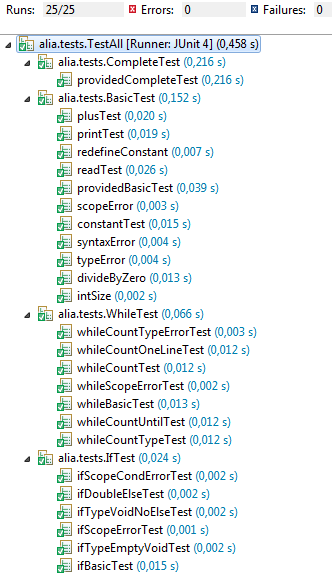
\includegraphics[scale=0.5]{images/testresults.png}
\end{center}



\section{Conclusion}
In this report we have described the Alia programming language. We have specified the features, the syntax, the context constraints and the semantics of the Alia language. Some of the problems that we faced during the construction as well as their solutions have been elaborated. We have also detailed for you the extra java classes constructed for the compiler and the full array of tests that have been made to verify the correctness of the language. Together these give you a good understanding of how the Alia programming language works both in programming and under the hood. For conclusions on the programming language itself. Alia is a language that contains all the functionality of the basic expression language, along with conditional statement and a while statement. Alia also features type inference, though procedures and functions have not yet been added. The extra functionality of functions and procedures is fairly major and for future work these should be the first to be added. The language offers a large amount of freedom as to what you want to write down, such as not having to hardly put any end of line delimiters except newlines and also not having to declare types for variables or constants. 

The construction of the Alia compiler was a very interesting learning experience. As everyone knows you put quite a lot of time into the final project of compiler construction, but you get rewarded with a new level of understanding of how programming languages work. It has been fun to be able to define your own programming language, and it is great to have an understanding of every stage of the compilation process, from code to actually executable instructions. Weighing all the gains against the time invested it was a very positive learning experience and definitely adds value to an education in computer science.

\newpage
\appendix
\section{Appendices}

\subsection{Responsibilities}
The following table makes clear who was responsible for what parts of the report.
\begin{tabular}{l | l}
Part & Person \\ \hline
Title page & Joost \\
Introduction & Fedor\\
Description & Joost \\
Problems & Fedor \\
Syntax, Context, Semantics & Fedor \\
Translation Rules & Joost\\
Java Code & Fedor\\
Tests & Joost \\
Conclusion & Fedor \\
\end{tabular}
%ANTLR LEXER
%ANTLR PARSER
%ANTLR TREEPARSER
%Een testprogramma (invoer/uitvoer)

\newgeometry{left=0.3cm,right=0.3cm,bottom=0.3cm,top=0.3cm}
\subsection{Lexer and parser}

\lstinputlisting[style=densecodenomargins, language=Assembly]{../src/alia/Alia.g}

\subsection{Checker}

\lstinputlisting[style=densecodenomargins, language=Assembly]{../src/alia/AliaChecker.g}

\subsection{Code Generator}

\lstinputlisting[style=densecodenomargins, language=Assembly]{../src/alia/AliaCodeGeneratorStringTemplate.g}

\subsection{String templates}

\lstinputlisting[style=densecodenomargins, language=Assembly]{../src/alia/jbc.stg}
\restoregeometry

\subsection{Example test program}
\label{testprogram}
The following test is designed to test most of the programming language functionalities.

\subsubsection{Alia code}
\begin{lstlisting}[style=muchcode]
ivar = begin
    ivar1 = ivar2 = 0
    read(ivar1, ivar2);
    print(ivar1, ivar2);
    const iconst1 = 1;
    const iconst2 = 2;
    ivar2 = ivar1 = +16 + 2 * -8;
    print(ivar1 < ivar2 && iconst1 <= iconst2,iconst1 * iconst2 > ivar2 - ivar1);
    ivar1 < read(ivar2) && iconst1 <= iconst2;
    ivar2 = print(ivar2) + 1;
  end + 1
bvar = begin
    bvar = false
    read(bvar);
    print(bvar);
    bvar = 12 / 5 * 5 + 12 % 5 == 12 && 6 >= 6;
    const bconst = true;
    print(!false && bvar == bconst || true != false);
  end && true;
cvar = begin
    cvar1 = 'c'
    read(cvar1);
    const cconst = 'c';
    cvar2 = 'z';
    print('a', cvar1 == cconst && cvar2 != 'b' || !true);
    'b';
  end;
print(ivar, bvar, cvar);

i = 0
z = 0
while x = 5; x > i do
  print(i)
  if z == 1 do
    z = 0
  elseif z == -1 do
    z = 1
  else
    z = -1
    i = i + 1
  end
end
\end{lstlisting}

\subsubsection{Test results}
The test program was run using the following input:
\begin{lstlisting}
30
-100
998
true
z
\end{lstlisting}

\noindent It resulted in the following output:
\begin{lstlisting}
30
-100
false
true
998
true
true
a
false
1000
true
b
0
1
1
1
2
2
2
3
3
3
4
4
4
\end{lstlisting}


\newgeometry{left=0.3cm,right=0.3cm,bottom=0.3cm,top=0.3cm}
\subsubsection{Jasmin bytecode}
\lstinputlisting[style=densecodecolumn, language=Assembly, multicols=2]{code/Complete.j}
\restoregeometry


% 
%%% End document
\end{document}
